\subsection 

Et accelerometer er et elektromekanisk apparat som anvendes til at måle accelerationskræfter. 
Det kan blandt andet registrere om et objekt bevæger sig opad, nedad og måle lineær acceleration\citep{Goodrich2013}. Enheden er målt i meter pr sekund i anden(m/s^2) eller i G kræfter (g). En enkel G kraft på jorden er tilsvarende til 9,8 m/s^2 , men det kan variere med elevation. \citep{Sparkfun}
Hvis outputtet af en sensor er vendt opad vil kraften være +1g, hvis outputtet af en sensor er horisontal er det tilsvarende 0g og hvis outputtet er vendt nedad vil det være tilsvarende -1g, som illusteret på figur \label{g}. 


\begin{figure}[H]
	\centering
	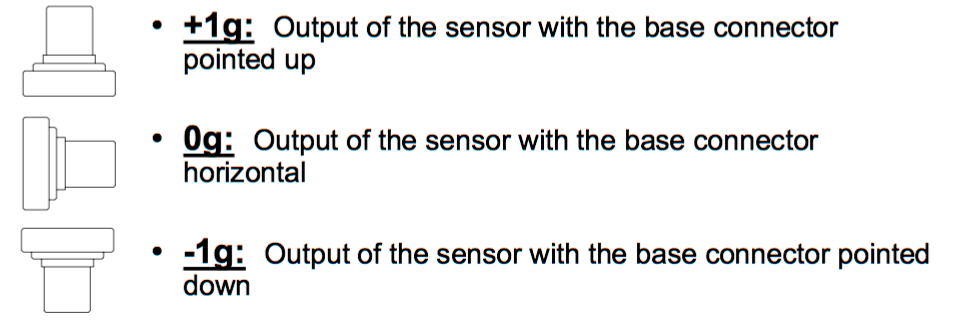
\includegraphics[scale=0.6]{figures/aProblemløsning/g.png}
	\caption{På figuren ses, antal af g afhængigt af hvilke retninger af accelerometeren måler\ . \cite{Unicef2016}}
	\label{fig:g}
\end{figure}



 
 På trods af størrelsen af et accelerometer, fungerer det på mange måder, hvor de mest anvendte er ved den piezoelektriske effekt og den kapacitance sensor. Den piezoelektriske effekt er den mest almindelige form for accelerometer. Denne anvender mikroskopiske krystalstrukturer, som stresses på grund af accelererende kræfter. Disse krystaller skaber en spænding ud fra stressen, hvor accelerometeret fortolker denne spænding til at bestemme hastigheden og retningen.
Den kapacistans\fixme{Kapacitans er et mål for, hvor meget elektrisk ladning som gemmes (eller separeres) for en given elektrisk spændingsforskel.} accelerometer, registrerer ændringer i kapistans mellem microstrukturer, som er placeret ved siden af enheden. Hvis en accelererende kraft bevæger en af disse strukturer, så vil kapacitansen blive ændret og accelerometeret vil fortolke denne kapacitans som spænding.  \citep{Goodrich2013}

Et accelerometer måler to former for acceleration, henholdsvis statisk og dynamisk, hvor de statiske kræfter inkluderer tyngdekraften og hvilken vinkelretningen enheden bliver tiltet hen. De dynamiske kræfter inkluderer hvilken retning enheden bevæger sig imod og dens vibrationer. \citep{Sparkfun,Engineering, Goodrich2013}

Man kan måle accelerationer i flere retninger ved af bruge flere end en accelerometre. \citep{Sparkfun}. Man kan måle acceleration af en akse, to akser(x,y) og tre akser (x,y,z) akser, hvor den sidste er den hyppigst anvendte. For eksempel har en bil to akser i en og de fleste smartphones har 3 akser. \citep{Sparkfun}

Man kan anvende AC og DC forsyninger til et accerlerometer, hvilket bestemmer typen af hardware og sætter en grænseflade for accelerometeren. \citep{Engineering}

I et AC-koblet accelerometer er outputtet AC, hvilket vil betyder at enheden ikke kan måle statisk acceleration såsom tyngdekraften, men kun dynamisk acceleration. 
En DC-koblet accelerometer kan måle nul hertz, og kan derfor anvendes til at måle både statisk og dynamisk acceleration. 



